% Introduction

\chapter{Introduction} % Main chapter title

\label{chapter:introduction}

%----------------------------------------------------------------------------------------

% Define some commands to keep the formatting separated from the content 
\newcommand{\keyword}[1]{\textbf{#1}}
\newcommand{\tabhead}[1]{\textbf{#1}}
\newcommand{\code}[1]{\texttt{#1}}
\newcommand{\file}[1]{\texttt{\bfseries#1}}
\newcommand{\option}[1]{\texttt{\itshape#1}}

%----------------------------------------------------------------------------------------
\section{Background}
The accretion of \enquote{Smart technology} and \enquote{Industry 4.0} has led to some revolutionary scientific development in the field of software development and networking. As a consequence, new features like the backend gateway applications are introduced to interconnect the physical or human-operated systems to monitor the data over the Internet, adding more operation reliability. The term \ac{IoT} has bridged the gap between the hardware and software worlds. A majority of embedded products used in the market has brought in the concept of compact design with minimal cost. In the last few decades, there has been a huge demand of cost effective embedded hardware and \ac{SoC} and it is rising exponentially with each passing year. 


The main focus area of an embedded design from the software development viewpoint is to choose an \ac{OS} for the binary image implementation of the target hardware where one can integrate custom applications and libraries effortlessly and embedded Linux seems to be the most preferable choice. One advantage of using Linux on the embedded platform is the reduced development time~\parencite{raghavan2005embedded}. Using a Linux based host development machine, one can easily develop and test more applications without having to fear about porting. With this thesis research, the in-depth understanding of the embedded Linux environment and the \ac{OE} framework is discussed, with reference to the Yocto project. The Yocto project is an open source project to implement the custom Linux based systems for an embedded hardware and \ac{OE} is the build framework for developing the embedded Linux distribution. It supports cross-compilation and provides rich set of development tools for the distribution build, with the flexibility to add additional software components according to organization needs. These software components are externally integrated into the build system. Few examples of the software components used within the department for its target embedded hardware, are the \ac{REST} \ac{API}, or REST API (application to transfer state of point resources in the form of \ac{JSON} to the endpoint via HTTP) or a web page configuration. 

At the initial project implementation stage, the software components are developed and maintained with the help of an independent release cycle. In industry terms, it is known as the \emph{Software Release Lifecycle}. It consists of the development, testing and delivery phase. These phases are critical for maintaining a good software quality. This paves way for DevOps and \ac{CI} and \ac{CD} pipeline which aids to greater functionalities like automated software build, testing and deployment of pipeline outputs. With each successful release, the implemented software components with proper version number and ready to be integrated into the target device. With software versioning, one has the opportunity to track changes to a particular software and recent substantial development done. 

To track a particular product lifecycle and \emph{its time-to-market}, the product development process also follow an independent release cycle, better known as a \emph{Product Release Lifecycle}. It involves stages like product planning, manufacturing, and testing to name a few among others. From the software development point of view, the end outcome of each development release is an output in the form of a delivery package. A software delivery package is the result of the build process. It contains the binary image, \ac{SDK}, licenses, release notes and other deliverables. Post release, \emph{external deliverables} in the delivery package such as the image file (ready to be flashed on the target hardware), release notes or the license files are delivered or procured by the customer and \emph{internal deliverables} like the original code base, testing results are just meant for project development purpose. 

The purpose of this thesis is also to study and implement a method to integrate one such internal deliverable into the product delivery package. The next few chapters present a more detailed overview of the software development process at both application and product levels and how software packages are integrated at the Yocto build level with preamble to the embedded Linux landscape.

%The Yocto Project documentation states the following 

%\vspace{0.5cm}
%\enquote{\emph{It contains the \ac{OE} Build System (BitBake and \ac{OE} Core) as well as a set of metadata to get started with building custom distribution}}~\parencite{Reference2}. 
%\vspace{0.5cm}



 %This paves way for DevOps, continuous integration and deployment which aids to greater functionalities to generate test reports, trigger email notification, and even upload to cloud artifactory (JFrog, GitHub).  Lastly, BitBake can also process the test reports at the event of build launch. In case, the test suite is not present, the quality of the software is compromised. Therefore, it is very critical for a project, that the test suite should be present and cover all the feature implementations before its final release. The next few chapters will present more detailed overview and practical scenarios why it is vital to have each application test reports in the build directory of the Linux distribution and discuss on ways to implement it via BitBake class files. 
%----------------------------------------------------------------------------------------

\section{Work Environment}

The master thesis work was conducted under the guidance of Nico Mueller and Martin Buschbeck from Bosch Thermotechnik GmbH, department of \emph{TT-RHC/XAT}. The company, situated in Lollar, is a wholly-owned subdivision of Robert Bosch GmbH.
The organization is prominent in the field of heating and energy efficient technologies and its product portfolio includes \textsc{HVAC} (heating,ventilation, and air conditioning) systems for instance energy-efficient hot water boilers. Bosch Thermotechnik GmbH have employed more than 14,000 people worldwide over 23 locations. 

The department \emph{TT-RHC/XAT} focuses on feature implementation of IT backend gateway for its business models. Gateway products such as the bus module \emph{MB LAN2} from Bosch Thermotechnik GmbH are already in market which connects to the heater/heat pump and can monitored via \emph{HomeCom Easy} mobile application. Another industrial application example is the \emph{Logamatic web KM300} gateway from Bosch Thermotechnik GmbH, marketed under the Buderus brand monitors the heating system remotely via the Internet and PC software. This leads to location-independent operation and monitoring. This thesis work also focuses on the software development part of one such gateway product for its \ac{EV} charging solution.

%----------------------------------------------------------------------------------------

\section{Problem Statement} \label{section:problemstatement}

The main advantage of using the Yocto project for building a custom Linux distribution is the fact that it is open-sourced and vendor independent. The Yocto project, together with the \ac{OE} build system provides a set of integrated tools to build a custom bootable Linux \ac{OS} stack. Most of the activity is done via \emph{Poky}, a reference distribution to set up the build environment. It is one of the core components that offers functionalities for a fully customizable Linux stack~\parencite{vaduva2015learning}. The build environment includes a comprehensive set of layers. Typically, these layers are just source control repositories that allow to organize the long list of providers such as metadata files like the configuration files, class files and special files called recipes meant to build and integrate software packages into the filesystem and compute tasks. To get started with custom distribution build, the metadata is parsed by BitBake (the build executor) during the build launch. Consequently, there are default layers with pre-installed recipes which are quintessential for building the base distribution and additional custom layers which includes recipes that are intended for a specific project depending on the company's customer requirement or the project. For example, recipes to define the custom software components like \ac{REST} \ac{API}, web configuration, among others are within a custom layer and executed during the Yocto build. 

The preceding information can also be verified with the current Yocto implementation within the department, for the integration of custom software applications and deployment of project deliverables for its target gateway product - ComModul - developed and marketed by Bosch Thermotechnik GmbH. To further accelerate the product release cycle, the Yocto build process is configured via an automated pipeline job containing all the pre and post build actions. To accomplish that, a build repository in the \ac{BDC} based platform (version control management (GitHub)) is configured with manifest that holds all the base and custom layer (Bosch layers and customer layers) information. At the time of execution, BitBake processes these layers, metadata executable and parses all the recipes files to build a custom Linux distribution and other essential directories. Finally, the deliverables are packaged in the form of a tarball and deployed to an upstream artifact repository licensed under Bosch Group. 

In the mentioned process, the current delivery package is missing the software test or validation reports integrated along with other project deliverables. These reports are an internal deliverable to the project and basically an organised summary of all the test objectives and results performed for \ac{QA} of software that needs to be integrated into the target product. A typical software test report will include all the passed or failed benchmark and performance test results taken against concrete validation suites\footnote{Accumulation of all the test cases}. So, after completion of the delivery phase in a product release cycle, there is no provision for the internal stakeholders\footnote{Internal Stakeholders: Embedded Developers, Testers, Project Managers} to refer to these reports under one single delivery package. They either need to refer to the test results against validation performed at the independent software release cycle, or manually run the validation suites, which is quite strenuous. For this reason, the best solution is to integrate the application test reports\footnote{The term application test reports or software package test reports or package test reports have been used interchangeably in this thesis, but it generally refers to a same meaning} into the delivery folder within the Yocto build directory during the execution of the build itself. This thesis aims to find a potential solution of this problem and in general the \emph{Software Integration at the Yocto level}. The goal of this research is to bring all the deliverables (internal and external) under one single umbrella of the Yocto delivery package. The architectural overview of the problem statement is illustrated with the help of Figure \ref{fig:Architectural summary of the Problem Statement}.



  %parses application recipes files and a Yocto image is created, followed by image testing and then the final deployment to an artifactory. The image is then ready to be delivered and mounted on an embedded product.




\begin{figure}
\centering
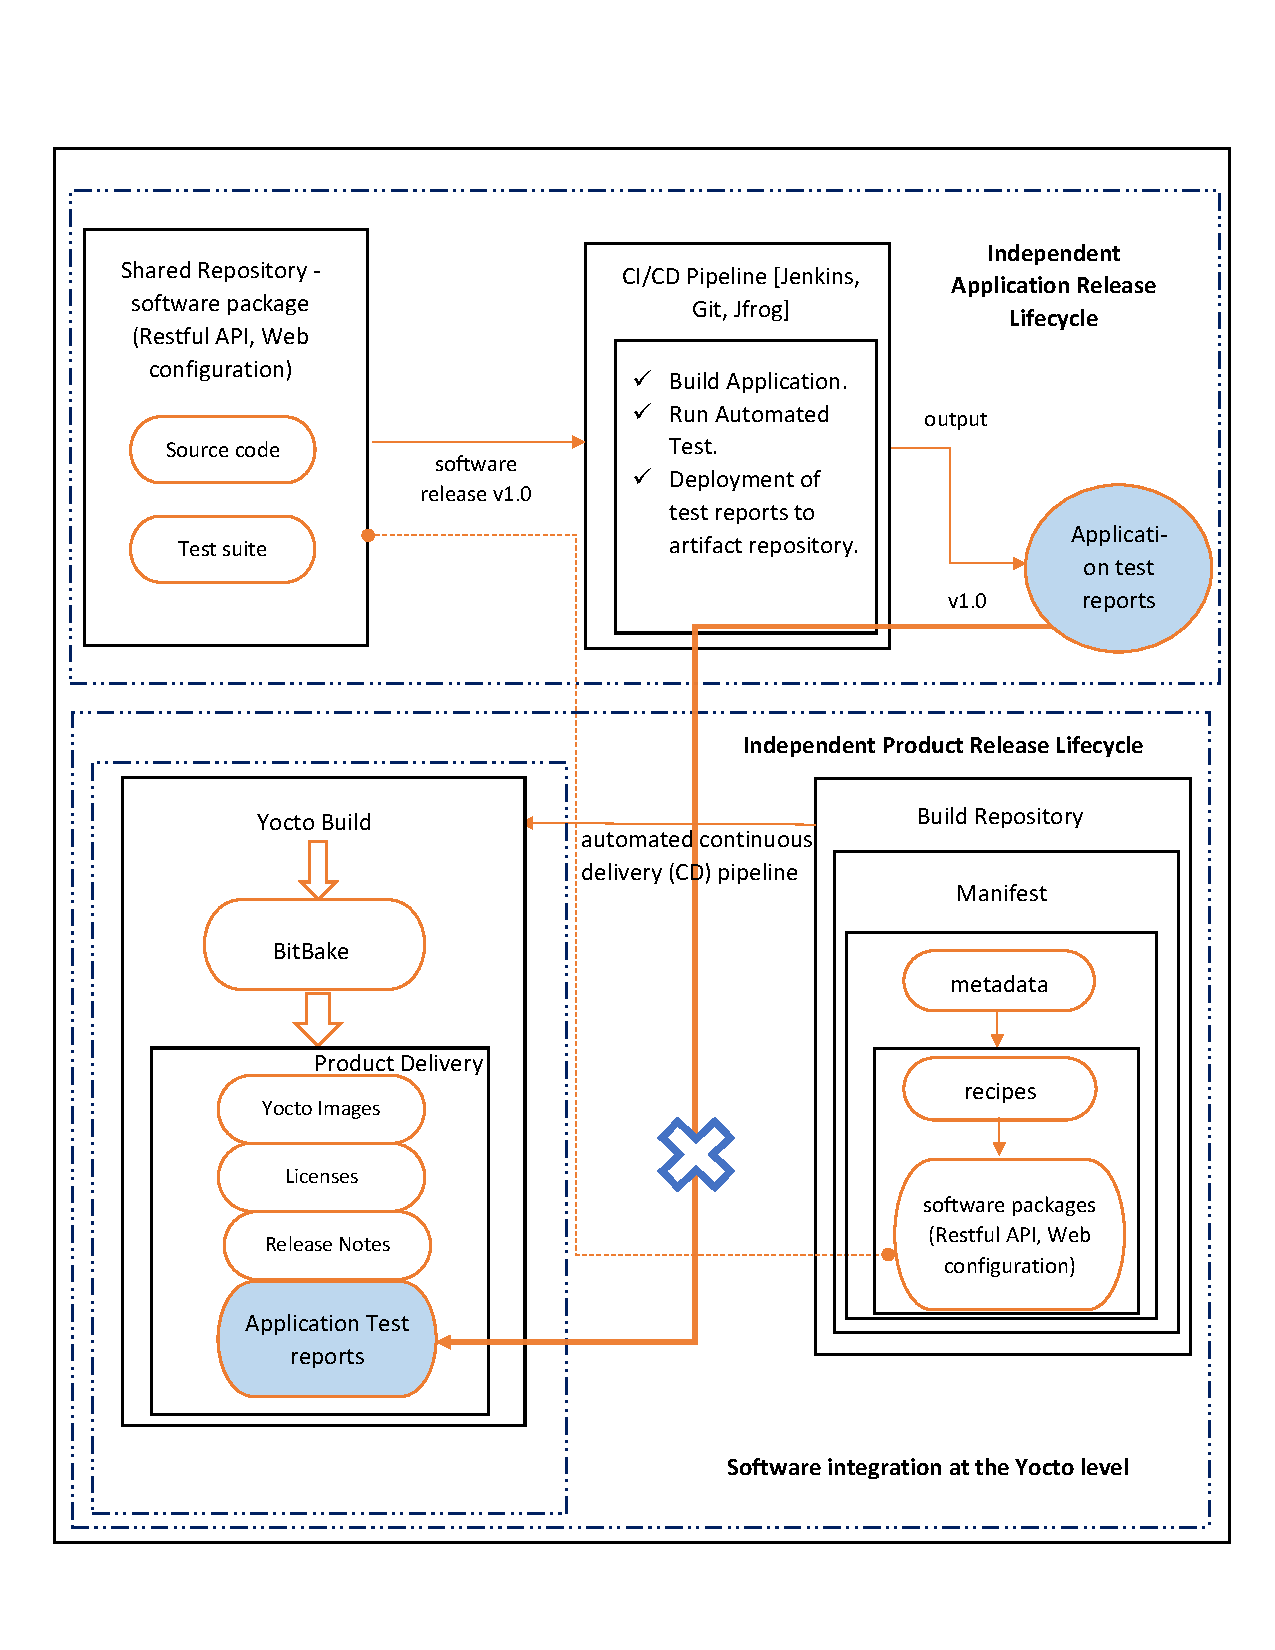
\includegraphics[scale=0.7]{figures/ThesisYocto.pdf}
\caption[Architectural summary of the problem statement]{Architectural summary of the problem statement}
\label{fig:Architectural summary of the Problem Statement}
\end{figure}


%----------------------------------------------------------------------------------------
\newpage
\section{Motivation}

The primary motivation behind the thesis work is to analyse the functionalities offered by BitBake and the Yocto project, in general and find a suitable approach to effectuate the Yocto level integration of internal deliverables. To conduct the research, few preliminary steps have been carried out.

In a potential \ac{SDLC}, a software application passes through many stages of build, planning, design and test, among others. In the scope of this thesis, the research tries to primarily automate the build and test process of an in-focus application - implemented and developed by Bosch Thermotechnik GmbH. Specifically, to achieve this, an automated \ac{CI} and \ac{CD} pipeline have to be configured with the help of an automation server or a \ac{CI} tool. This brings the benefit that the application will be continuously integrated, build and tested against each software versions without the involvement of any manual effort. A \ac{CI} tool is more like an orchestrator, connected to the version control system to automate the build, test, and deployment process of software packages~\parencite{pathania2017learning}. It can be executed manually with just a click or configured nightly, or weekly depending upon the project release plan. The preliminary work is also implemented on one such \ac{CI} tool, \emph{Jenkins} licensed under Robert Bosch GmbH. The generated test report or the validation results are then deployed as a tar artifact to a Bosch internal delivery platform like JFrog artifactory. The main use of the JFrog platform is to store the project deliverables such as the project binaries, images, application test reports, licences. Later, with each release of the software application, 
an implementation concept will be developed to fetch the test reports and integrate them into the Yocto delivery package during the build process.

The secondary motivation of the thesis work is to address the key concerning area and current shortcoming defined in Section~\ref{section:problemstatement} by identifying and analyzing the the existing work done in the area of developing an embedded Linux distribution with the Yocto project within the department. The implemented custom layers and recipes must be examined in aspect of installing the custom software packages or application. Thereafter, the thesis can study the current concept of how BitBake interprets the application recipe and configure a feature implementation to integrate the test reports as well. Finally, few validations should be in place to evaluate the effectiveness of the work and how it improves the overall release cycle of the embedded gateway product. The identified and mentioned tools used for the thesis purpose are all licensed under Robert Bosch GmbH.

Besides, all the mentioned concerns, the thesis also figure out a way to improve the release lifecycle of the implemented software components and demonstrate an implementation concept to automate the current release process in terms of project version control. The paper identifies the following five key questions and strive to look for the best solution.
  
\vspace{0.2cm}
\begin{itemize}

\item {Question 1: What is software integration and delivery and how to automate this process considering one software component in-focus within the department ?}
\item {Question 2: How to automate the software release process in respect to version control ?}
\item {Question 3: Which internal deliverable is the focus of this thesis ?}
\item {Question 4: How to integrate the aforementioned internal deliverable into the product delivery package at the Yocto level ?}
\item {Question 5: How does the thesis work improves the overall Product release lifecycle ?}
\end{itemize}

\noindent\keyword{Note on Intellectual Property}  \hspace{0.5cm}The software implementation and target gateway product comprises the intellectual property of Bosch Group. The customer name or neither the original code base have been published in this thesis work. Therefore, the presented implementation code chunks are distorted from the actual code base but at the same time demonstrate the aforementioned concerned issue on the subject matter in-focus.

%----------------------------------------------------------------------------------------

\section{Thesis Structure}

Given the questions mentioned above, the thesis work have been organised into few following chapters to answer it.

  
\begin{itemize}
\item \keyword{Chapter 1} - This chapter address question 1 in the first section and reflects on the relevant basics about modern software development process with highlights to software integration and delivery. The following section of the chapter discusses the basic terminologies used in embedded Linux landscape and Yocto project. It explains the implementation terms in detail, for the readers to understand the hypotheses solution about how to address the problem statement.

%used in the research paper quite often and also in areas of application testing phase with a spotlight on terms such as test automation, continuous integration and deployment pipeline, containerization. addressed the question,  

\item \keyword{Chapter 2} - The preliminary work, carried out to reach the goal of the thesis is described in this chapter. It mainly finds ways to automate the process of software integration and answers the second part of the concerned question 1. The pipeline methodology is discussed in this chapter with the help of modern DevOps tools, in use within the department. 

\item  \keyword{Chapter 3} - The chapter identifies an area of improvement related to the ongoing software release process within the department. The analysis covers the key area of concern and the involvement of manual effort and tedious work if the current release process exists. Concurrently, a solution approach is outlined by presenting a corresponding implementation to mitigate the identified concern in software release control. 

\item  \keyword{Chapter 4} - The relative major and minor key solution for the descriptive problem statement is elaborated in this chapter. The analysis of the existing software package integration concept at the Yocto level is studied and a corresponding way of integrating the test reports of the software packages to the yocto delivery package is outlined.

\item \keyword{Chapter 5} - This chapter validates the qualitative research and implemented solution from Chapters 3 and 4.

\item \keyword{Chapter 6} - Finally with this chapter, this thesis work is summarized and all possible future work in this area is drawn.


\end{itemize}

%on the implementation of the class file and other changes made to the recipe. The research outlines the development of a custom class file that extends the BitBake fetch module to obtain the automated test reports from a source path and unpack to the deploy directory in the build system.

%----------------------------------------------------------------------------------------
\section{State of the art}

The contemporary software development process is noted in many publications and scientific papers, of which few notable publications have been considered to answer the purpose of this thesis. It would be an injustice not to mention the quality of the work Alexandre and Tom have put in their research paper~\parencite{8721084} about terminologies used in software versioning and package releases. It appears that the importance of automated builds to integrate software components within projects inside the organization has been considered by many existing research papers. Mathias~\parencite{6802994} discusses how continuous integration is more than a set of practices to increase a product's \emph{time-to-market} and its customer value.




Most of the existing literature about how to get started with the landscape of Yocto project explores the subject matter in considerable depth. The thesis gives special attention to the brilliant work produced by Rudolf~\parencite{Reference1}, and Otavio and Daiane~\parencite{salvador2014embedded} which analyses the Yocto build system in their individual publications and presents examples that can be applied to the real-life configuration. This thesis follows a practical approach based on the implementation concepts outlined in these books regarding the integration of software packages and building a customizable Linux OS stack with the Yocto project and the \ac{OE} build system. Some scientific research papers take advantage of the Yocto project and its key components to developing a custom OS based on its purpose. For example, Toomas Aleksander~\parencite{veromannembedded}, in his research publication, mentions developing a custom Linux distribution for gateway devices in smart home environments. One more journal paper from Mahendra and Abhishek Kumar~\parencite{swain2015design} published, in which the Yocto based embedded Linux device is implemented for the purpose of voice calling. Massimo, Cristiano, and Alessandro~\parencite{violanteembedded} report the Yocto project layer model in their work and the custom metadata layers implemented for a given set of software packages required in the Magneti Marelli organization. As highlighted in these previous literature work, layers and other metadata files play an important role in the integration of deliverables ( both internal and external). This thesis gathers all the mentioned literature to consider a concrete implementation idea to demonstrate the solution.



 
A certain section of this thesis discusses about automating the release cycle of software projects, based on the \texttt{standard-version} tool already present in the industry under permissible open software license by the \ac{ISC}. The tool takes care of the algorithm behind a software version bump. This thesis takes the support of the mentioned tool and configures it with an automation server. However, the in-depth study of the algorithm working behind this tool is not covered in this paper. This paper identifies a current shortcoming in aspect to the manual involvement in software release within the department and highlights implementation ways to automate it.










%The are few notable publications on the one hand the book Software Product Lines in Action: The Best Industrial Practice in Product Line Engineering [Linden, Schmid and Rommes 2007] in the industrial













\clearpage\null\thispagestyle{empty}



%Major companies have welcomed the modern approaches of application development by driving automation into projects. The commencement of DevOps practice has brought in a significant impact on development speed and time to market for a product. The aim of the work is to make use of \ac{CI}, \ac{CD} pipeline to test various software applications and analyze test reports. Furthermore, these test reports are packaged into an artifact, which can then be fetched into the Yocto build host with the help of BitBake and Yocto classes. The thesis is organized into the following chapters: